\section{Date: 2026-08-06}
\noindent \textbf{Series ID: NAFTARECP} 

\noindent This series is titled OECD based Recession Indicators for NAFTA Area from the Peak through the Period preceding the Trough (DISCONTINUED) and has a frequency of Monthly. The units are +1 or 0 and the seasonal adjustment is Not Seasonally Adjusted.The observation start date is 1947-03-01 and the observation end date is 2022-08-01.The popularity of this series is 1. \\ 

\noindent \textbf{Series ID: BOPBCAA} 

\noindent This series is titled Balance on Current Account (DISCONTINUED) and has a frequency of Annual. The units are Billions of Dollars and the seasonal adjustment is Not Seasonally Adjusted.The observation start date is 1960-01-01 and the observation end date is 2013-01-01.The popularity of this series is 6. \\ 

\subsection{Raw Regression}
\noindent Regresses the two series against each other directly. A significant result here can come just as easily from both series sharing a long-run trend as from any real relationship.

\begin{center}
\begin{tabular}{lclc}
\toprule
\textbf{Dep. Variable:}         & value\_fred\_BOPBCAA & \textbf{  R-squared:         } &     0.005   \\
\textbf{Model:}                 &         OLS          & \textbf{  Adj. R-squared:    } &    -0.014   \\
\textbf{Method:}                &    Least Squares     & \textbf{  F-statistic:       } &    0.2814   \\
\textbf{Date:}                  &   Thu, 06 Aug 2026   & \textbf{  Prob (F-statistic):} &    0.598    \\
\textbf{Time:}                  &       13:27:58       & \textbf{  Log-Likelihood:    } &   -371.18   \\
\textbf{No. Observations:}      &            54        & \textbf{  AIC:               } &     746.4   \\
\textbf{Df Residuals:}          &            52        & \textbf{  BIC:               } &     750.3   \\
\textbf{Df Model:}              &             1        & \textbf{                     } &             \\
\textbf{Covariance Type:}       &      nonrobust       & \textbf{                     } &             \\
\bottomrule
\end{tabular}
\begin{tabular}{lcccccc}
                                & \textbf{coef} & \textbf{std err} & \textbf{t} & \textbf{P$> |$t$|$} & \textbf{[0.025} & \textbf{0.975]}  \\
\midrule
\textbf{const}                  &    -188.9963  &       40.873     &    -4.624  &         0.000        &     -271.014    &     -106.979     \\
\textbf{value\_fred\_NAFTARECP} &      35.6291  &       67.161     &     0.531  &         0.598        &      -99.139    &      170.398     \\
\bottomrule
\end{tabular}
\begin{tabular}{lclc}
\textbf{Omnibus:}       & 12.191 & \textbf{  Durbin-Watson:     } &    0.065  \\
\textbf{Prob(Omnibus):} &  0.002 & \textbf{  Jarque-Bera (JB):  } &   13.569  \\
\textbf{Skew:}          & -1.223 & \textbf{  Prob(JB):          } &  0.00113  \\
\textbf{Kurtosis:}      &  3.210 & \textbf{  Cond. No.          } &     2.43  \\
\bottomrule
\end{tabular}
%\caption{OLS Regression Results}
\end{center}

Notes: \newline
 [1] Standard Errors assume that the covariance matrix of the errors is correctly specified.

\begin{figure}
\centering
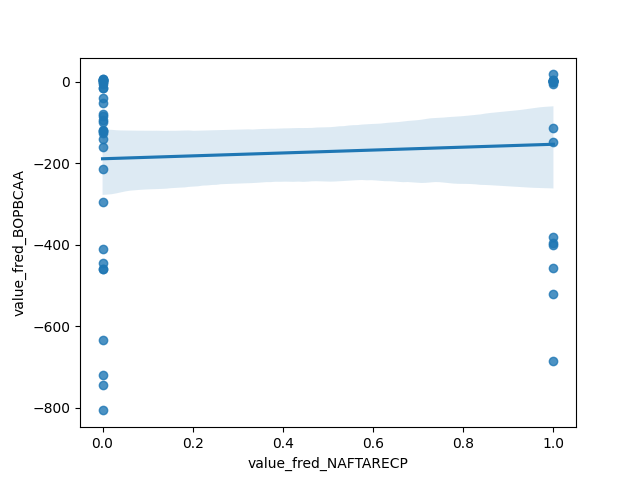
\includegraphics[scale = 0.9]{plots/plot_2026-08-06.png}
\caption{Raw Regression Plot for 2026-08-06}
\end{figure}
\newpage
\subsection{Detrended Regression}
\noindent Regresses the residuals of each series after removing its own linear time trend, so a shared trend can no longer drive the result on its own. A relationship that stays significant here is better evidence of a genuine link between the two series.

\begin{center}
\begin{tabular}{lclc}
\toprule
\textbf{Dep. Variable:}                    & value\_fred\_BOPBCAA\_detrended & \textbf{  R-squared:         } &     0.000   \\
\textbf{Model:}                            &               OLS               & \textbf{  Adj. R-squared:    } &    -0.019   \\
\textbf{Method:}                           &          Least Squares          & \textbf{  F-statistic:       } &   0.02165   \\
\textbf{Date:}                             &         Thu, 06 Aug 2026        & \textbf{  Prob (F-statistic):} &    0.884    \\
\textbf{Time:}                             &             13:27:58            & \textbf{  Log-Likelihood:    } &   -340.93   \\
\textbf{No. Observations:}                 &                  54             & \textbf{  AIC:               } &     685.9   \\
\textbf{Df Residuals:}                     &                  52             & \textbf{  BIC:               } &     689.8   \\
\textbf{Df Model:}                         &                   1             & \textbf{                     } &             \\
\textbf{Covariance Type:}                  &            nonrobust            & \textbf{                     } &             \\
\bottomrule
\end{tabular}
\begin{tabular}{lcccccc}
                                           & \textbf{coef} & \textbf{std err} & \textbf{t} & \textbf{P$> |$t$|$} & \textbf{[0.025} & \textbf{0.975]}  \\
\midrule
\textbf{const}                             &    7.162e-12  &       18.522     &  3.87e-13  &         1.000        &      -37.167    &       37.167     \\
\textbf{value\_fred\_NAFTARECP\_detrended} &      -5.6739  &       38.562     &    -0.147  &         0.884        &      -83.055    &       71.707     \\
\bottomrule
\end{tabular}
\begin{tabular}{lclc}
\textbf{Omnibus:}       &  8.580 & \textbf{  Durbin-Watson:     } &    0.207  \\
\textbf{Prob(Omnibus):} &  0.014 & \textbf{  Jarque-Bera (JB):  } &    7.858  \\
\textbf{Skew:}          & -0.877 & \textbf{  Prob(JB):          } &   0.0197  \\
\textbf{Kurtosis:}      &  3.646 & \textbf{  Cond. No.          } &     2.08  \\
\bottomrule
\end{tabular}
%\caption{OLS Regression Results}
\end{center}

Notes: \newline
 [1] Standard Errors assume that the covariance matrix of the errors is correctly specified.

\begin{figure}
\centering
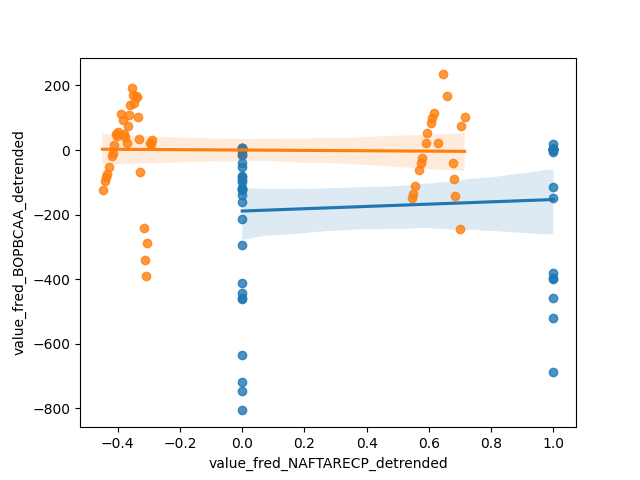
\includegraphics[scale = 0.9]{plots/plot_2026-08-06_detrended.png}
\caption{Detrended Regression Plot for 2026-08-06}
\end{figure}
\newpage
